\section{Divide and Conquer} 

  \begin{definition}[Divide and Conquer Algorithms]
    The general idea is two steps: 
    \begin{enumerate}
      \item Divide an input into smaller instances of the same problem. The simplest form is merge sort. 
      \item Conquer/solve these smaller instances, which takes less time. 
      \item Merge/Combine the smaller solutions into the original, bigger solution. 
    \end{enumerate}
    This is usually recursive, but does not need to be. 
  \end{definition}

  It has its applications in the most elementary operations, in sorting and multiplication. To prove correctness, we use induction by proving the correctness of the base case and then the inductive step to show that there is an invariant. 

\subsection{Recursive Algorithms and Recurrence Relation}

  I assume that the reader is familiar with recursive algorithms. Now to evaluate the runtime of a recursive algorithm, one must implicitly solve for the runtime of its recursive calls, and we can visualize it. 

  \begin{figure}[H]
    \centering 
    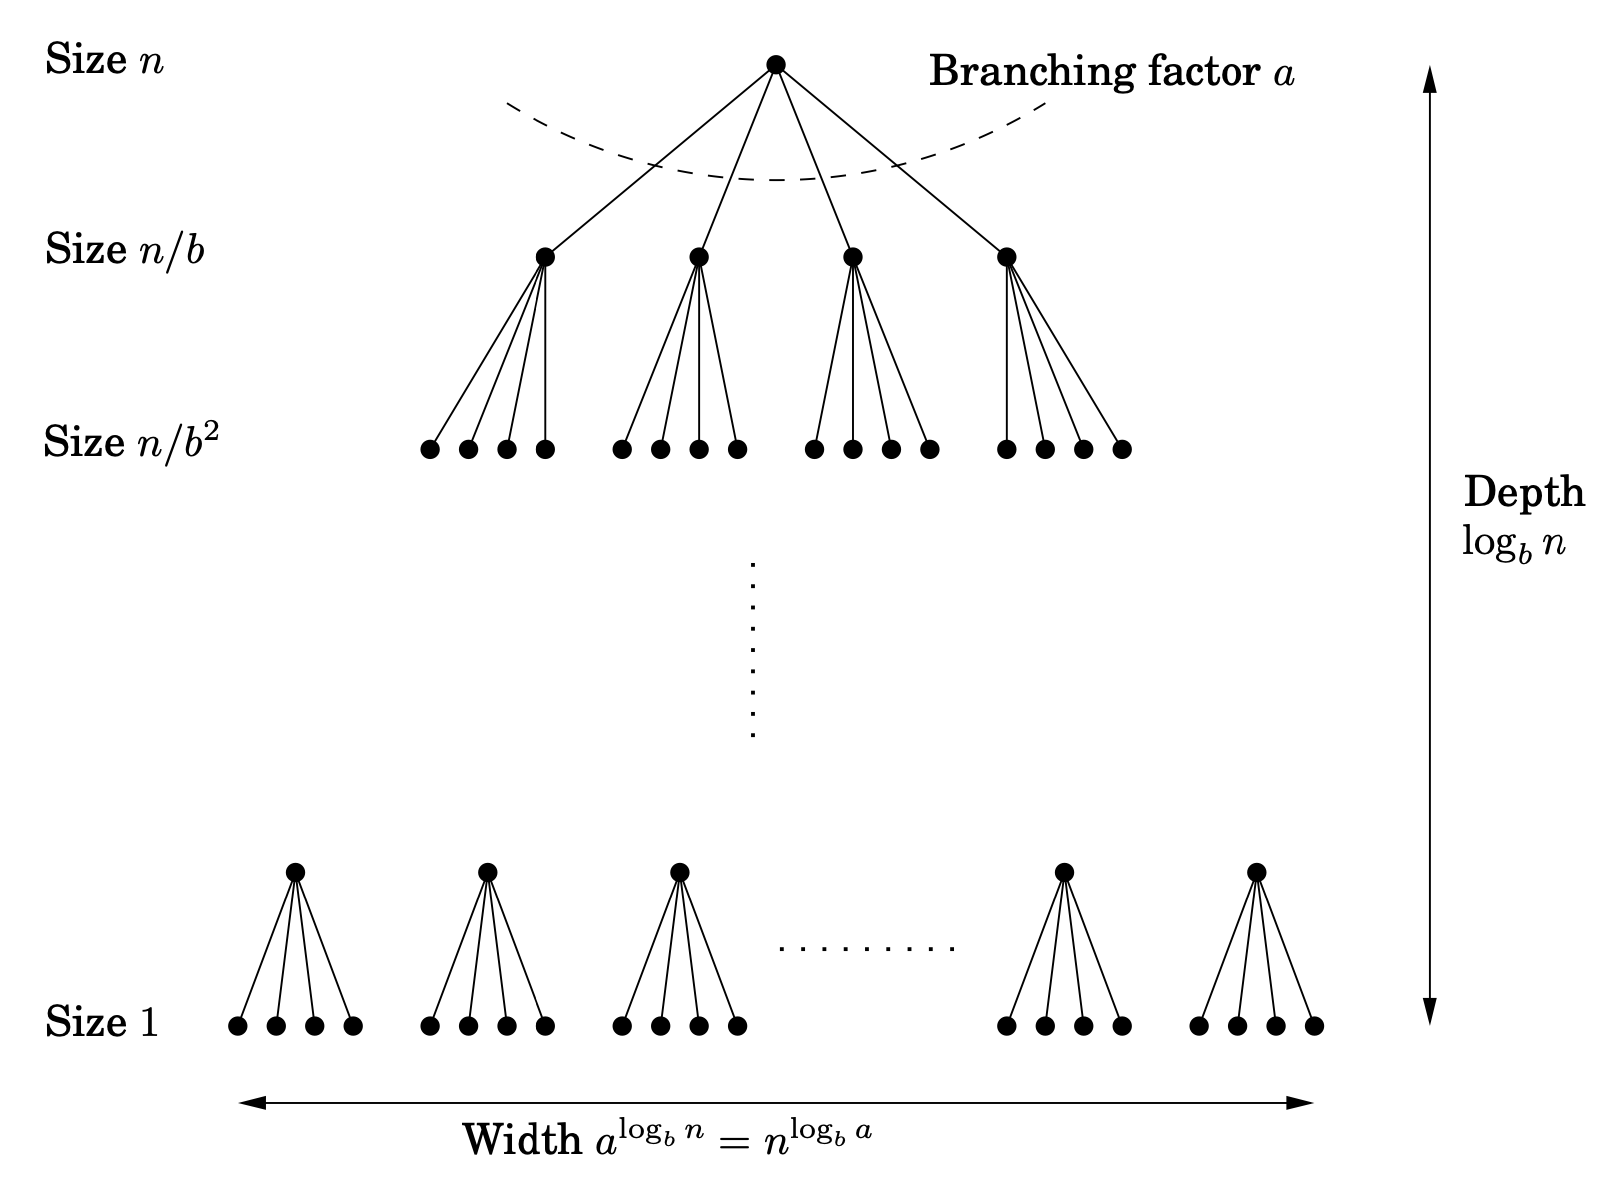
\includegraphics[scale=0.4]{img/branching.png}
    \caption{} 
    \label{fig:branching}
  \end{figure}

  An important theorem for divide-and-conquer algorithms is 

  \begin{theorem}[Master Theorem]
    Given a recurrence relation of form 
    \begin{equation}
      T(N) = a T(N/b) + O(N^c)
    \end{equation}
    then the following holds 
    \begin{align}
      a > b^c & \implies T(N) = O(N^{\log_b a}) \\
      a = b^c & \implies T(N) = O(N^c \log{N}) \\
      a < b^c & \implies T(N) = O(N^c) 
    \end{align}
  \end{theorem}
  \begin{proof}
    To intuit this, see that if $a > b^c$, then there arises a lot of subproblems, so our complexity is greater. If $a < b^c$, then we have few subproblems and can get a better runtime. If $a = b^c$, we get somewhere in between. To actually solve this, we can just unravel the recurrence to get the infinite series 
    \begin{align}
      T(N) & = a T(N/b) + O(N^c) \\
           & = a^2 T(N/b^2) +  N^c \bigg( \frac{a}{b^c} + 1 \bigg) \\
           & =  N^c \bigg( 1 + \frac{a}{b^c} + \frac{a^2}{b^{2c}} + \ldots \bigg)
    \end{align}
    So, if $a < b^c$, then even as $N \rightarrow \infty$, the sum is finite, so it is of order $O(N^c)$. If $a = b^c$, then the series is just $1 + \ldots + 1$, which scales on the order of $O(\log_2 {N})$. If $> 1$, then we have to calculate the last term, which contributes to our runtime and overpowers $c$.  
    
    Therefore, if $a$ is large, our algorithm will have an exponential number of subproblems and will be bottlenecked by the. 
  \end{proof}

\subsection{Merge Sort and Counting Inversions}

  \begin{algo}[Merge Sort]
    Merge sort is the first instance. 
    \begin{algorithm}[H]
      \caption{Merge Sort}
      \label{alg:merge_sort}
      \begin{algorithmic}
        \Require{Array \texttt{nums}}
        \Function{MergeSort}{\texttt{nums}}
          \State \texttt{n = len(nums)}

          \If{\texttt{n < 2}} \Comment{base case}
            \State \Return{nums}
          \EndIf
          \State \texttt{mid = n // 2} 
          \State \texttt{left\_sorted = MergeSort(nums[:mid])} \Comment{Divide into left half}
          \State \texttt{right\_sorted = MergeSort(nums[mid:])} \Comment{Divide into right half}

          \State \texttt{res = [0] * n} 
          \State \texttt{i = j = k = 0} 
          \While{\texttt{k < n}} \Comment{Merge the sorted subarrays}
            \If{\texttt{j == len(right\_sorted) or left\_sorted[i] < right\_sorted[j]}}
              \State \texttt{res[k] = left\_sorted[i]} \Comment{We should add the next element from left array}
              \State \texttt{i += 1} \Comment{if it is smaller or if right array is filled already}
            \Else 
              \State \texttt{res[k] = right\_sorted[j]}
              \State \texttt{j += 1}
            \EndIf 
            \State \texttt{k += 1}
          \EndWhile

          \State \Return{\texttt{res}}
        \EndFunction
      \end{algorithmic}
    \end{algorithm}
    The recurrence relation for the runtime is as follows. Let $T(n)$ represent the worst-case runtime of \texttt{MergeSort} of size $n$. Then, we have 
    \begin{equation}
      T(n) = 2 \cdot T(n/2) + O(n)
    \end{equation}
    Consisting of two recursive calls with input size $n/2$ and then the merge step which is $O(n)$. But if we take a look at this, we have 
    \begin{align}
      T(n) & = 2 \cdot T(n/2) + O(n) \\
           & = 2 \cdot \big( 2 \cdot T(n/4) + O(n/2)) + O(n) \\
           & = 4 \cdot T(n/4) + O(n) + O(n) 
    \end{align}
    and the number of times $O(n)$ is added up is $\log{n}$, meaning that this recurrence relation turns into $O(n \log{n})$. 
  \end{algo}

  \begin{definition}[Inversions]
    Given two lists of ranked items, say 
    \begin{align}
      \text{Alice}: & a > b > c > d > e \\
      \text{Bob}: & b > d > a > e > c
    \end{align}
    We want to measure the dissimilarity between two rankings by counting the number of \textit{inversions}, which are pairs of items for which open persons orders the opposite of the other (e.g. $a, b$ for above).\footnote{Also known as Kendall-Tau distance in statistics.} So how many inversions are there? We can do this in $\Theta(n^2)$ by explicitly looking at all $n$ pairs. Without loss of generality, we can assume that the first list is sorted simply by bijectively relabeling these elements for both lists. Therefore, the set of inversions is defined to be 
    \begin{equation}
      \{(i, j) \text{ s.t. } i < j \text{ and } \texttt{A[i] > A[j]}\}
    \end{equation}
  \end{definition}

  \begin{algo}[Counting Inversions]
    The idea is very similar. By assuming that the first list is sorted, we can simply count the number of inversions in a single list $A$.  
    \begin{lstlisting}
      A = 5 6 1 3 4 8 2 7
    \end{lstlisting}
    \begin{enumerate}
      \item In the divide step, we count all inversions in $A_l, A_r$, which are the left and right sides of $A$, \textit{and} we sort $A_l, A_r$ to add additional structure.  
        \begin{lstlisting}
          1 3 5 6 | 2 4 7 8
        \end{lstlisting}
      \item In the conquer step, we merge them linearly but every time we add an element from $A_r$ into our result, this reveals that there are $k$ additional inversions added where $k$ is the number of elements left in $A_l$ to add.  
    \end{enumerate}
    \begin{algorithm}[H]
      \caption{Counting Inversions}
      \label{alg:inversions}
      \begin{algorithmic}
        \Require{Array \texttt{nums}}
        \Function{Inversions}{\texttt{nums}}
          \State \texttt{n = len(nums)}

          \If{\texttt{n < 2}} \Comment{base case}
            \State \Return{nums}
          \EndIf
          \State \texttt{mid = n // 2} 
          \State \texttt{left\_sorted, left\_invs = Inversions(nums[:mid])} \Comment{Divide into left half}
          \State \texttt{right\_sorted, right\_invs = Inversions(nums[mid:])} \Comment{Divide into right half}

          \State \texttt{res = [0] * n} 
          \State \texttt{i = j = k = 0} \Comment{left, right, and combined index}
          \State \texttt{inv = 0} \Comment{number of inversions}
          \While{\texttt{k < n}} \Comment{Merge the sorted subarrays}
            \If{\texttt{j == len(right\_sorted) or left\_sorted[i] < right\_sorted[j]}}
              \State \texttt{res[k] = left\_sorted[i]} \Comment{We should add the next element from left array}
              \State \texttt{invs += len(left\_sorted - i)} \Comment{Increment inversions by \# of elems in left array}
              \State \texttt{i += 1} \Comment{if it is smaller or if right array is filled already}
            \Else 
              \State \texttt{res[k] = right\_sorted[j]}
              \State \texttt{j += 1}
            \EndIf 
            \State \texttt{k += 1}
          \EndWhile

          \State \Return{\texttt{res, inv + left\_invs + right\_invs}}
        \EndFunction
      \end{algorithmic}
    \end{algorithm}
    The recursion relation is still 
    \begin{equation}
      T(n) = 2 \cdot T(n/2) + O(1) + O(n) \implies O(n \log{n})
    \end{equation}
  \end{algo}

\subsection{Selection and Quick Sort} 

  The next problem is a generalization of finding the median of an array, which we present can be done in $O(n)$ time \textit{on average}. It turns out that that this idea of choosing a pivot and then dividing and conquering happens often in general selection and sort algorithms.    

  \begin{algo}[Select kth Largest Element from Unsorted Array]

    \begin{algorithm}[H]
      \caption{Find Kth Largest Element}
      \label{alg:kth_largest}
      \begin{algorithmic}
        \Require{Array of numbers nums, integer k where 1 <= k <= length(nums)}
        \State
        \Function{FindKthLargest}{nums, k}
            \If{length(nums) = 1} \Comment{Base case: if array has only one element}
                \State \Return nums[0]
            \EndIf
            
            \State pivot $\gets$ $\lfloor$length(nums)/2$\rfloor$ \Comment{Select middle element as pivot}
            \State left $\gets$ [ ] \Comment{Unsorted array for elements smaller than pivot}
            \State right $\gets$ [ ] \Comment{Unsorted array for elements larger than pivot}
            \State n\_pivots $\gets$ 0 \Comment{Count of elements equal to pivot}
            
            \For{each n in nums} \Comment{Start filling in the arrays}
                \If{n = nums[pivot]}
                    \State n\_pivots $\gets$ n\_pivots + 1
                \ElsIf{n $\leq$ nums[pivot]}
                    \State left.append(n)
                \Else
                    \State right.append(n)
                \EndIf
            \EndFor
            
            \If{length(right) $\leq$ k - 1 \textbf{and} length(left) $\leq$ length(nums) - k}
              \State \Return nums[pivot] \Comment{Found the $k$th element which was in the middle in n\_pivots}
            \ElsIf{length(right) $\geq$ k}
              \State \Return \Call{FindKthLargest}{right, k} \Comment{Largest is in the array of bigger numbers.}
            \Else
              \State \Return \Call{FindKthLargest}{left, k - length(right) - n\_pivots} \Comment{Largest is in the array of smaller numbers.}
            \EndIf
        \EndFunction
      \end{algorithmic}
    \end{algorithm}
  \end{algo}

  \begin{algo}[Quick Sort]
    
    \begin{algorithm}[H]
      \caption{Quicksort Algorithm}
      \label{alg:quicksort}
      \begin{algorithmic}
        \Require{Array A of comparable elements}
        \State
        \Function{Quicksort}{A, low, high}
            \If{low < high}
                \State p $\gets$ \Call{Partition}{A, low, high} \Comment{Get pivot position}
                \State \Call{Quicksort}{A, low, p - 1} \Comment{Sort left subarray}
                \State \Call{Quicksort}{A, p + 1, high} \Comment{Sort right subarray}
            \EndIf
        \EndFunction
        \State
        \Function{Partition}{A, low, high}
            \State pivot $\gets$ A[high] \Comment{Choose rightmost element as pivot}
            \State i $\gets$ low - 1 \Comment{Index of smaller element}
            
            \For{j $\gets$ low to high - 1} \Comment{Scan through array}
                \If{A[j] $\leq$ pivot}
                    \State i $\gets$ i + 1 \Comment{Increment index of smaller element}
                    \State swap A[i] and A[j] \Comment{Swap current element with pivot}
                \EndIf
            \EndFor
            \State swap A[i + 1] and A[high] \Comment{Put pivot in its correct position}
            \Return i + 1 \Comment{Return pivot's final position}
        \EndFunction
      \end{algorithmic}
    \end{algorithm}
  \end{algo}

\subsection{Closest Pair of Points} 

  The next problem simply takes a series of points and calculates the closest pair of points. This can be done trivially in $O(N^2)$ by taking all combinations, but with clever divide and conquer, we can reduce this down. The idea is that we want to divide them into a left and a right side, which we can sort in $O(N \log{N})$ and find the median in $O(1)$. This now reduces to computing the closest pair of points in each $N/2$ half. If we can find the closest pair in each half, then we must compare it to all pairs of points across the halves, meaning that we must do $(N/2)^2$ comparisons again, leading to 
  \begin{equation}
    T(N) = 2 T(N/2) + O(N^2)
  \end{equation}
  which isn't any better than $O(N^2)$. But imagine that we found that the smallest distance of the left and right were $\delta_1, \delta_2$, then for each point in the left side, we don't have to check all $N/2$ points on the right. 

  \begin{figure}[H]
    \centering
    \begin{tikzpicture}[
      scale=0.7,
      y=0.6cm, % Vertical compression
      point/.style={circle, fill=black, draw=black, minimum size=0.12cm, inner sep=0},
      distanceline/.style={-, thick, blue}
    ]
      % Dashed vertical line dividing the space
      \draw[dashed, orange!70!brown] (0,-5) -- (0,5);
      
      % Random points on left side
      \node[point] (p1) at (-4,2) {};
      \node[point] (p2) at (-2,4) {};
      \node[point] (p3) at (-2,1) {};
      \node[point] (p4) at (-3,-1) {};
      \node[point] (p5) at (-1,-2) {};
      \node[point] (p6) at (-0.7,0) {};
      \node[point] (p7) at (-1,-4) {};
      \node[point] (p8) at (-0.8,-3) {};
      
      % Random points on right side
      \node[point] (p9) at (1,3) {};
      \node[point] (p10) at (3,4) {};
      \node[point] (p11) at (2,0) {};
      \node[point] (p12) at (3.5,2) {};
      \node[point] (p13) at (2.5,-1) {};
      \node[point] (p14) at (3.8,-1) {};
      \node[point] (p15) at (1,-3) {};
      \node[point] (p16) at (2,-4) {};
      
      % Distance markers with labeled distances
      \draw[distanceline] (p1) -- (p2) node[midway, left] {$\delta_1$};
      \draw[distanceline] (p13) -- (p14) node[midway, below] {$\delta_2$};
      
    \end{tikzpicture}
    \caption{Set of points with two measured distances $\delta_1$ and $\delta_2$.}
    \label{fig:point-distances}
  \end{figure}

  We just have to check those with distance at most $\delta = \min\{\delta_1, \delta_2\}$ from each point. Furthermore, we can discard all points that are too far away from the boundary. However, all $N$ points could like in the relevant space, leading to $O(N^2)$ computations of distance. 

  \begin{figure}[H]
    \centering
    \begin{tikzpicture}[
      scale=0.7,
      y=0.6cm, % Vertical compression
      point/.style={circle, fill=black, draw=black, minimum size=0.12cm, inner sep=0},
      distanceline/.style={-, thick, blue},
      boundary/.style={dashed, green!70!black, thin},
      center/.style={dashed, orange!70!brown, thick}
    ]
      % Add shading on background layer
      \begin{scope}[on background layer]
        % Green shading for discard regions
        \fill[green!10] (-6,-5) rectangle (-3,5);
        \fill[green!10] (3,-5) rectangle (6,5);
        
        % Red shading for relevant region
        \fill[red!10] (-3,-5) rectangle (3,5);
      \end{scope}
      
      % Vertical lines
      \draw[center] (0,-5) -- (0,5);
      \draw[boundary] (-3,-5) -- (-3,5);
      \draw[boundary] (3,-5) -- (3,5);
      
      % Random points on left side
      \node[point] (p1) at (-4,2) {};
      \node[point] (p2) at (-2,4) {};
      \node[point] (p3) at (-2,1) {};
      \node[point] (p4) at (-3,-1) {};
      \node[point] (p5) at (-1,-2) {};
      \node[point] (p6) at (-0.7,0) {};
      \node[point] (p7) at (-1,-4) {};
      \node[point] (p8) at (-0.8,-3) {};
      
      % Random points on right side
      \node[point] (p9) at (1,3) {};
      \node[point] (p10) at (3,4) {};
      \node[point] (p11) at (2,0) {};
      \node[point] (p12) at (3.5,2) {};
      \node[point] (p13) at (2.5,-1) {};
      \node[point] (p14) at (3.8,-1) {};
      \node[point] (p15) at (1,-3) {};
      \node[point] (p16) at (2,-4) {};
      
      % Distance markers with labeled distances
      \draw[distanceline] (p1) -- (p2) node[midway, left, blue] {$\delta_1$};
      \draw[distanceline] (p13) -- (p14) node[midway, below, blue] {$\delta_2$};
      
      % Curly braces
      \draw[black, thick, decorate, decoration={brace, amplitude=10pt, mirror}] (-3,-4) -- (0,-4);
      \draw[black, thick, decorate, decoration={brace, amplitude=10pt, mirror}] (0,-4) -- (3,-4);
      \node[black, font=\small, anchor=west] at (0,-5.5) {$\delta = \min(\delta_1, \delta_2)$};
    \end{tikzpicture}
    \caption{Closest pair algorithm with divide-and-conquer approach: only points within $\delta$ distance of the dividing line need to be checked for cross-boundary minimum distances. Note that if the closest pair consists of one point being in LHS and the other in the RHS of the red line, then it must lie in between the two green lines. }
    \label{fig:closest-pair-algorithm}
  \end{figure}

  Therefore, we want to incorporate vertical distances and tile our relevant space into square of side length $\delta/2$.  

  \begin{figure}[H]
    \centering 
    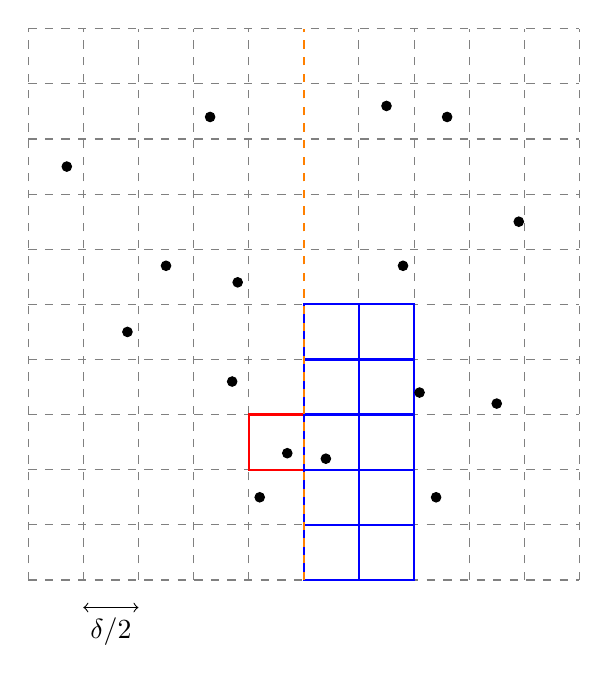
\begin{tikzpicture}[
      scale=0.7,
      y=1.0cm, % No vertical compression
      point/.style={circle, fill=black, draw=black, minimum size=0.12cm, inner sep=0},
      grid/.style={dashed, gray, thin}
      ]
      % Draw grid lines
      % Horizontal grid lines
      \foreach \y in {-5,-4,...,5} {
        \draw[grid] (-5,\y) -- (5,\y);
      }
      % Vertical grid lines
      \foreach \x in {-5,-4,...,5} {
        \draw[grid] (\x,-5) -- (\x,5);
      }
      
      % Add vertical middle line in orange
      
      % Add red box on the 3rd row from bottom and 5th column
      \draw[red, thick] (-1,-3) rectangle (0,-2);

      \draw[blue, thick] (0,-1) rectangle (1,-0);
      \draw[blue, thick] (1,-1) rectangle (2,-0);
      \draw[blue, thick] (0,-2) rectangle (1,-1);
      \draw[blue, thick] (1,-2) rectangle (2,-1);
      \draw[blue, thick] (0,-3) rectangle (1,-2);
      \draw[blue, thick] (1,-3) rectangle (2,-2);
      \draw[blue, thick] (0,-4) rectangle (1,-3);
      \draw[blue, thick] (1,-4) rectangle (2,-3);
      \draw[blue, thick] (0,-5) rectangle (1,-4);
      \draw[blue, thick] (1,-5) rectangle (2,-4);

      \draw[orange, thick, dashed] (0,-5) -- (0,5);
      
      % Add label for grid square side
      \draw[<->] (-4,-5.5) -- (-3,-5.5) node[midway, below] {$\delta/2$};
      % Perturbed points on left side
      \node[point] (p1) at (-4.3,2.5) {};
      \node[point] (p2) at (-1.7,3.4) {};
      \node[point] (p3) at (-2.5,0.7) {};
      \node[point] (p4) at (-3.2,-0.5) {};
      \node[point] (p5) at (-1.3,-1.4) {};
      \node[point] (p6) at (-1.2,0.4) {};
      \node[point] (p7) at (-0.8,-3.5) {};
      \node[point] (p8) at (-0.3,-2.7) {};
      
      % Perturbed points on right side
      \node[point] (p9) at (1.5,3.6) {};
      \node[point] (p10) at (2.6,3.4) {};
      \node[point] (p11) at (1.8,0.7) {};
      \node[point] (p12) at (3.9,1.5) {};
      \node[point] (p13) at (2.1,-1.6) {};
      \node[point] (p14) at (3.5,-1.8) {};
      \node[point] (p15) at (0.4,-2.8) {};
      \node[point] (p16) at (2.4,-3.5) {};
    \end{tikzpicture}
    \caption{We claim that each square has at most 1 point, since if there were two, then their distance would be less than $\delta / \sqrt{2}$, which contradicts the distance between the two points being greater than $\delta$. Therefore given a point, we only need to check a bounded constant. The number of points on the other side with distance $\leq \delta$ is at most $10$. If we are more careful, we can reduce the number down to $7$. } 
    \label{fig:closest_point3}
  \end{figure}

  It turns out that we just need to compute $5N = (N/2) \cdot 10$ distances at most, and now our question reduces to how do we find these 5 points? Well we can first sort the points on the left and right by their y-coordinates, so we can just take a sliding window that encapsulates these points on the right for every on the left. The pointers of the sliding window should point to a point where the y-coordinate is at most $\delta$ away, and this can be done in constant time. Therefore, our recurrence relation is  

  \begin{equation}
    T(N) = 2 T(N/2) + O(N \log{N}) \implies T(N) = O(N \log^2 {N})
  \end{equation}
  
  This sorting along the y-coordinates is a bottleneck, but we can just shove this into the recursion step by telling the left and right to not just return the $\delta_1, \delta_2$, but also the points sorted in the y-coordinate. Then at the end of the merge, we also merge the lists $L, R$ so that $S = L \cup R$ is sorted on $y$, which also takes $O(N)$ and doesn't add extra runtime on the merge step. This reduces the runtime to $O(N \log{N})$. 

  \begin{algo}[Closest Pair of Points]
    The next problem simply takes a series of points and calculates the closest pair of points. This can be done trivially in $O(N^2)$ by taking all combinations, but with clever divide and conquer, we can reduce this down. 
    \begin{algorithm}[H]
      \caption{Closest Pair of Points}
      \label{alg:closest_pair}
      \begin{algorithmic}
        \Require{$N$ points $\{(x_i, y_i)\}$.}
        \State 
        \Function{ClosestPair}{P} 
          \State Sort points by x-coordinate. \Comment{Bottleneck of $O(N \log{N})$}
          \If{len(P) = 2} 
            \State \Return $d(p_1, p_2)$, sorted $P$ by y-coord
          \EndIf

          \State $\delta_1, L \gets$ ClosestPair($P_L$)
          \State $\delta_2, R \gets$ ClosestPair($P_R$)
          \State $\delta = \min\{\delta_1, \delta_2\}$ 
          \State min $\gets \delta$
          \For{$l \in L$ s.t. distance to boundary $\leq \delta$} \Comment{$O(N)$ iterations}
            \State $W_l \gets \delta$-window of points in $R$ around $l$. \Comment{Can be done in $O(1)$ using sliding window.}
            \For{$r \in W_l$} \Comment{This is bounded by $O(10)$}
              \If{$d(p, l) < \delta$} 
                \State min $\gets d(p, l)$
              \EndIf
            \EndFor
          \EndFor

          \State merge $L$ and $R$ into sorted $S$ \Comment{O(N)} 

          \State \Return{min, S}
        \EndFunction
      \end{algorithmic}
    \end{algorithm}
  \end{algo}

\subsection{Multiplication}

  \subsubsection{Karatsuba Algorithm}


  \subsubsection{Strassen Algorithm}

    We can solve matrix multiplication of two $N \times N$ matrices in a slightly more clever way than $O(N^3)$. Note that we can take the $2 \times 2$ block form of matrices $A, B$ and multiply them to get $C = AB$, where 
    \begin{align}
      C_{11} & = A_{11} B_{11} \cdot A_{12} B_{21} \\ 
      C_{12} & = A_{11} B_{12} \cdot A_{12} B_{22} \\ 
      C_{21} & = A_{21} B_{11} \cdot A_{22} B_{21} \\ 
      C_{22} & = A_{21} B_{12} \cdot A_{22} B_{22} 
    \end{align}

    This requires us to compute a total of $8$ $N/2 \times N/2$ multiplications and 4 additions, each of which is $O(N^2)$. Therefore, our recurrence relation is 
    \begin{equation}
      T(N) = 8 T(N/2) + O(N^2)
    \end{equation}

    Using the master theorem, we find that $a = 8 > 2^2 = b^c$, so our runtime is $O(N^{\log_{b} a}) = O(N^3)$, which brings us right back to where we started. The problem with this is that $a = 8$, which is large. If we could get $a = 7$, then this would be an improvement. We want to reduce this number of multiplications, and we can do this using the Strassen algorithm, which uses the following values.  
    \begin{align*}
      P_1 &= (a_{11} + a_{22}) (b_{11} + b_{22}) \\
      P_2 &= (a_{21} + a_{22}) b_{11} \\
      P_3 &= a_{11} (b_{12} - b_{22}) \\
      P_4 &= a_{22} (b_{21} - b_{11} \\
      P_5 &= (a_{11} + a_{12}) b_{22} \\
      P_6 &= (a_{21} - a_{11}) (b_{11} + b_{12}) \\
      P_7 &= (a_{12} - a_{22}) (b_{21} + b_{22}) 
    \end{align*}
    Then, we claim that we the entries of $C$ are 
    \begin{align*}
        c_{11} &= P_1 + P_4 - P_5 + P_7 \\
        c_{12} &= P_3 + P_5 \\
        c_{21} &= P_2 + P_4 \\
        c_{22} &= P_1 + P_3 - P_2 + P_6
    \end{align*}
    So we have reduced 8, 4 mult/add to 7, 18 mult/add. Addition is cheap and the number of additions is bounded, so now we have decreased $a$ to $7$.\footnote{We can reduce it even further, down to $2.37$. Whether $O(N^2)$ is possible is an open problem. } We can then solve the new recurrence relation 
    \begin{equation}
      T(N) = 7 T(N/2) + O(N^2) \implies O(N^{\log_2 7}) \approx O(N^{2.81})
    \end{equation}

\subsection{Polynomial Multiplication with Fast Fourier Transform}

  Given as inputs $2$ degree $N$ polynomials, 
  \begin{align}
    A(x) & = a_0 + a_1x + a_2x^2 + \ldots + a_{n-1}x^{n-1} \\
    B(x) & = b_0 + b_1x + b_2x^2 + \ldots + b_{n-1}x^{n-1} 
  \end{align}
  we want to multiply them to $C(x) = A (x) B(x)$ defined 
  \begin{equation}
    C(x) = c_0 + c_1x + \cdots + c_{2n-2}x^{2n-2} 
  \end{equation}
  Clearly, we must multiply every coefficient in $A$ with $B$, which takes $O(N^2)$ time. It is also called the convolution operation. 
  \begin{align*}
    &\text{Convolution of } (a_0, a_1, \ldots, a_{n-1}) \text{ and } (b_0, b_1, \ldots, b_{n-1}) \\[1em]
    &c_0 = a_0 b_0 \\
    &c_1 = a_0 b_1 + a_1 b_0 \\
    &c_2 = a_0 b_2 + a_1 b_1 + a_2 b_0 \\
    &c_3 = a_0 b_3 + a_1 b_2 + a_2 b_1 + a_3 b_0 \\
    &\vdots \\
    &c_{2n-2} = a_{n-1} b_{n-1}
  \end{align*}

  We can actually compute this convolution of two vectors in $O(N \log{N})$ time using the FFT algorithm. Let's ease into this idea. 

  \begin{lemma}[Evaluating a Polynomial at x]
    If we are given an $x$ and want to evaluate $A(x)$, we can just incrementally evaluate the terms up each degree in $O(N)$ time. 

    \begin{algorithm}[H]
      \caption{Evaluate polynomial $A(x)$ at $x=p$}
      \begin{algorithmic}[1]
      \State $S \gets a_0$
      \State $R \gets x$
      \For{$i = 1, 2, \ldots, n-1$}
          \State $S \gets S + a_i \cdot R$
          \State $R \gets R \cdot x$
      \EndFor
      \end{algorithmic}
    \end{algorithm}
  \end{lemma}

  Great, we can make some progress, but what does this have to do with finding the actual polynomial? Recall that from the fundamental theorem of algebra, a set of $n+1$ points will uniquely determine a $n$th degree polynomial. This at first glance doesn't help, since evaluating all $n+1$ points is $O(n^2)$, and even if we did, this doesn't really tell us how to reconstruct the polynomial in some fast time (e.g. matrix inversion won't work). But note that if we have a 1st degree polynomial, then evaluating it at $\pm1$ will retrieve the whole polynomial back
  \begin{equation}
    f(x) = a_0 + a_1 x \implies \begin{cases} f(+1) & = a_0 + a_1 \\ f(-1) & = a_0 - a_1 \end{cases} \implies \begin{cases} a_0 & = \frac{1}{2} \big( f(+1) + f(-1) \big) \\ a_1 = \frac{1}{2} \big( f(+1) - f(-1) \big) \end{cases}
  \end{equation}

  We can think of this as sort of our base case. For $N$th degree polynomials, we can divide it into a even and odd powers part. 
  \begin{align}
    A(x) & = a_0 + a_1 x + a_2 x^2 + \ldots \\ 
         & = (a_0 + a_2 x^2 + a_4 x^4) + x (a_1 + a_3 x^2 + a_5 x^4 + \ldots ) \\
         & = A_{\mathrm{even}} (x^2) + x A_{\mathrm{odd}} (x^2) 
  \end{align}
  where each of the splits have degree $N/2$. Then we want to evaluate the even and odd parts. 

  Let's jump ahead and focus on the problem of evaluating $A(x)$ of degree $N$ at the $N$th roots of unity. 

  \begin{example}
    For $N = 4$, we evaluate at $\pm 1, \pm i$. 
    \begin{equation}
      A(x) = (a_0 + a_2 x^2) + x (a_1 + a_3 x^2) 
    \end{equation}
    which gives us 
    \begin{align}
      A(+1) & = A_e (+1) + A_o (+1) \\ 
      A(-1) & = A_e (+1) - A_o (1) \\ 
      A(+i) & = A_e (-1) + i A_o (-1) \\ 
      A(-i) & = A_e (-1) - i A_o (-1) 
    \end{align}
    Note that even though we had $\pm i$ evaluated on $A$, they were all squared in each split so evaluating the 4th of unity, which we denote $U(4)$, has been reduced to finding $U(2)$ for each of the left and right polynomials. 
  \end{example}

  Therefore, to evaluate $A$ of degree $N$ at $U(N)$, it suffices to evaluate $A_e, A_o$ each at $U(N/2)$, followed by combing them using addition and multiplication, which turns out to be $O(N)$. Therefore, for each step of evaluating $A$, you 
  \begin{enumerate}
    \item evaluate $A_e$ and $A_o$, and 
    \item then combine them in $\Theta(N)$ time
  \end{enumerate}

  \begin{algo}[Evaluate Nth Degree Polynomial at Nth Roots of Unity]
    
    \begin{algorithm}[H]
      \label{alg:unity}
      \begin{algorithmic}
        \Require{}
        \State 
        \Function{Func}{x}
        \EndFunction
      \end{algorithmic}
    \end{algorithm}
  \end{algo}

  Therefore, we have divided the problem of evaluating over $U(N)$ to be 
  \begin{equation}
    T(N) = 2 T(N/2) + O(N) \implies T(N) = O( N \log{N}) 
  \end{equation}

  So we have shown that in general, evaluating $N$ points of a polynomial takes $O(N^2)$ time, but if you're clever about what points to evaluate, you can get $O(N \log N)$. 

  Now going back to the original problem, we can evaluate $A(u), B(u)$ for $u \in U(N)$, and then multiply them to get $C(u)$. Great. Now to reconstruct the polynomial using the roots of unity, it turns out that there is a method in $O(N \log{N})$ time as well. 

